
\subsubsection{17.11.14}

\begin{enumerate} 
	\item The time of beginning and ending of the congregation:
	18:00 - 20:40
	\item Purposes of the congregation:
	\begin{enumerate}
		\item Improve the construction of bucket.
		
		\item Test the working of bucket.
		
	\end{enumerate}
	
	\item Work, that has been done:
	\begin{enumerate}
		\item Bucket was improved:
		\begin{enumerate}
			\item Inside the tube was placed plastic bottle. Tube was extended by another one bottle for more accuracy of throwing the balls into the basket.
			
			\item At the bottom part of bucket they was fixed plastic stripes which help to balls to enter the pipe and not get stuck.
			
			\item The bottom of bucket was bended as a boat. It was made in order balls doesn't fall outside the bucket during the raise of it.
			
			\item In bottom part of the bucket left only hole at center for hit the balls inside. It also allows to reduce risk of falling balls outside the bucket during the rise.
			
		\end{enumerate}
		
	    \begin{figure}[H]
			\begin{minipage}[h]{0.47\linewidth}
				\center{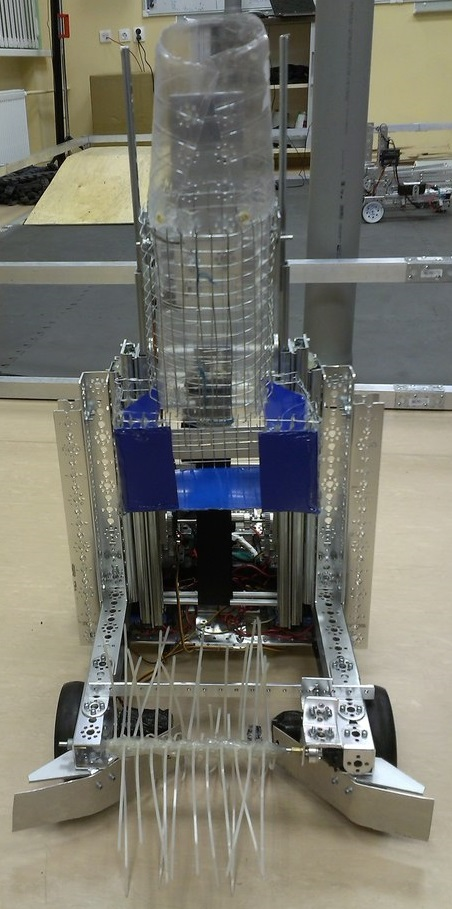
\includegraphics[scale=0.3]{days/17.11.14/images/01}}
				\caption{Bucket in vertical position}
			\end{minipage}
			\hfill
			\begin{minipage}[h]{0.47\linewidth}
				\center{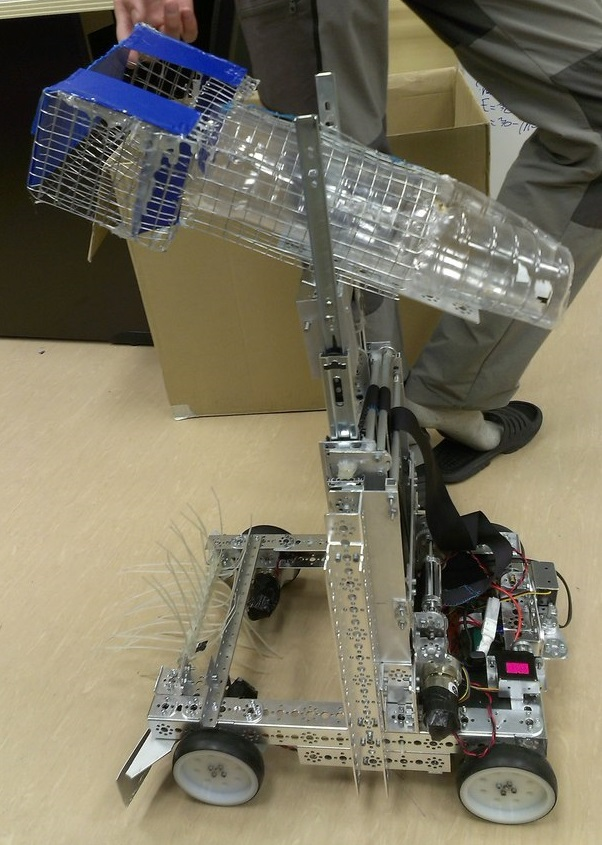
\includegraphics[scale=0.3]{days/17.11.14/images/02}}
				\caption{Bucket in turned position}
			\end{minipage}
		\end{figure}
		
		
		\item The bucket was tested manually. Bucket can fill 2 big and 3 small balls. It is enough because at every big ball there is 3 small. Balls doesn't fall outside the bucket during the rise.
		
		
	\end{enumerate}
	
	\item Results:
	\begin{enumerate}
		\item Construction of the bucket was finished.
		
		\item During the test no problems detected.
		
	\end{enumerate}
	
	\item Tasks for the next congregations:
	\begin{enumerate}
		\item Test the bucket with help programme.
		
	\end{enumerate}     
\end{enumerate}
\fillpage

